\chapter{Dasar Desain Schematic dan PCB}

\section{Tujuan}
\begin{enumerate}
    \item Belajar mendesain sirkuit elektronik menggunakan software
    \item Mengetahui fungsi setiap komponen dan cara implementasinya
    \item Memahami proses menyusun komponen agar bisa digunakan bersamaan dengan komponen lain untuk melakukan fungsi tertentu
    \item Untuk memperkenalkan beberapa konsep dasar dan teknik laboratorium dalam mendesain schematic dan PCB
    \item Mendesain rangkaian PCB yang nantinya dapat dicetak menjadi komponen dengan fungsi tertentu
\end{enumerate}


\section{Dasar Teori}
Sebelum menyusun hardware dan komponen kecil seperti IC di breadboard dan
bahkan mensoldernya di PCB, ada baiknya kita melakukannya di software terlebih dahulu agar
kita bisa mengecek kompatibilitas tiap komponen dan mengecekknya secara virtual
disamping secara rinci mengetahui fungsi setiap komponen yang hendak kita gunakan
nantinya. Pada praktikum kali ini akan digunakan software Fusion360 untuk mendesain
schematic dan PCB yang nantinya akan diprint, selain memiliki fitur yang mumpuni, banyak
tutorial cara penggunaan serta tersedia banyak library komponen yang sering kali dipakai
pada project arduino, MCU, dan elektronika.

Praktikan diharapkan sudah membaca secara rinci modul instalasi Fusion360 dan mencoba fitur-fitur dasarnya dengan membuat schematic sederhana. Pada kali ini praktikan
akan arahkan untuk membuat rangkaian schematic dan board menggunakan MCU ESP-8266
dan beberapa komponen lain yang bisa diprogram menjadi alat IoT sederhana.

Kesalahan yang seringkali dijumpai pada proses desain PCB yaitu routing yang
membingunkan bagi pemula, atau jika sudah melakukan routing namun desainnya sulit
dipahami oleh pengguna lain, maka dari itu untuk memudahkan pembacaan schematic
digunakanlah fitur name dan label, hal ini digunakan untuk menyederhanakan desain tanpa
mengurangi sedikitpun fungsi utama sirkuit tersebut. Untuk mengecek apakah komponen
tersebut telah terkoneksi, gunakan fitur SHOW dan arahkan kursor mouse ke arah kabel yang
ingin dicek, dan jika kabel pada ujung dan pangkal sama-sama ter-highlight maka komponen
yang mendapat suplai daya tersebut sudah pasti terkoneksi dengan benar.

\section{Tugas Pendahuluan}
\begin{enumerate}
    \item Install Fusion 360 pada Laptop masing-masing anggota kelompok
    \item Buat jalur PCB rangkaian regulator lm7805 dari schematic yang telah disediakan pada folder praktikan
    \item Buatlah Wiring Schematic Minimum System ESP8266! Caranya seperti dibawah.
\end{enumerate}

\section{Wiring Schematic Minimum System ESP8266}
Untuk Tugas Pendahuluan, akan dibuat sebuah desain schematic Minimum System untuk menjalankan 
chip ESP8266 sehingga dapat dihubungkan dengan komputer dan dilakukan flash program ke ROM nya. 
Minimum System ESP8266 ini akan disuply dayanya dengan tegangan sebesar 3,3 Volt yang diatur 
oleh 3,3-Voltage Regulator nya. Untuk dapat menyambungkan ESP8266 dengan host computer yang 
dapat melakukan flash programnya maka digunakan connector JST 4 PIN TTL to USB, 
sebagai penghubung koneksi ESP8266 dengan host computer. Minimum System dari ESP8266 juga memiliki 
2 switch yang digunakan untuk melakukan Reset dan Flash.
\begin{enumerate}
    \item Untuk memulai membuat project klik \textbf{New Project} di kiri atas dan beri nama sesuai yang kalian inginkan
        \begin{figure}[H]
            \centering
            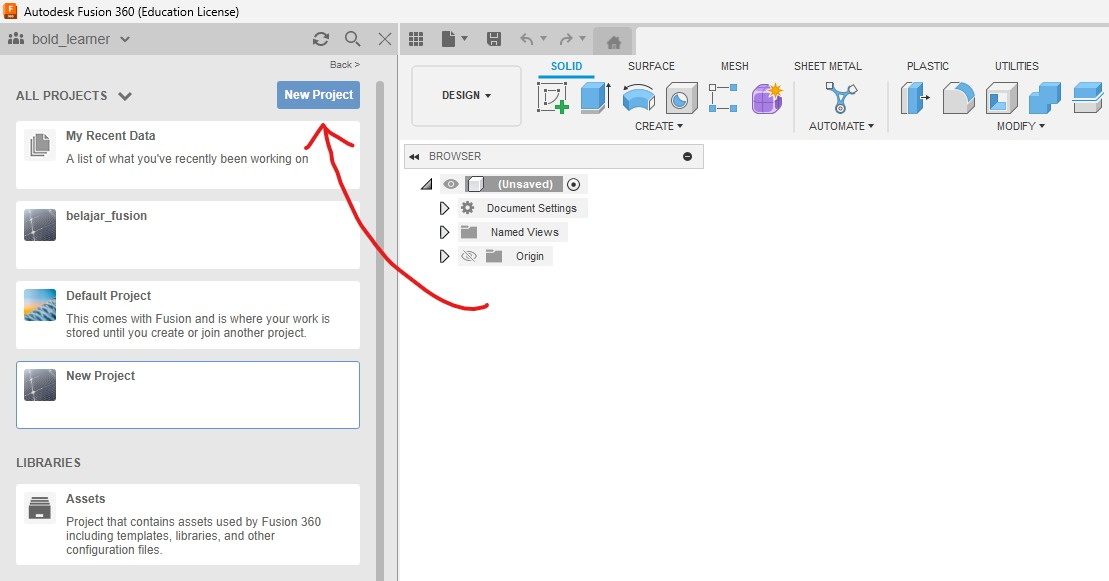
\includegraphics[width=0.6\linewidth]{P1/img/gambar1.jpeg}
            \caption{buat project baru} 
            \label{fig:buat project baru}
        \end{figure}
    \item Selanjut nya buka project space yang telah kalian buat pada window di bagian kiri
        \begin{figure}[H]
            \centering
            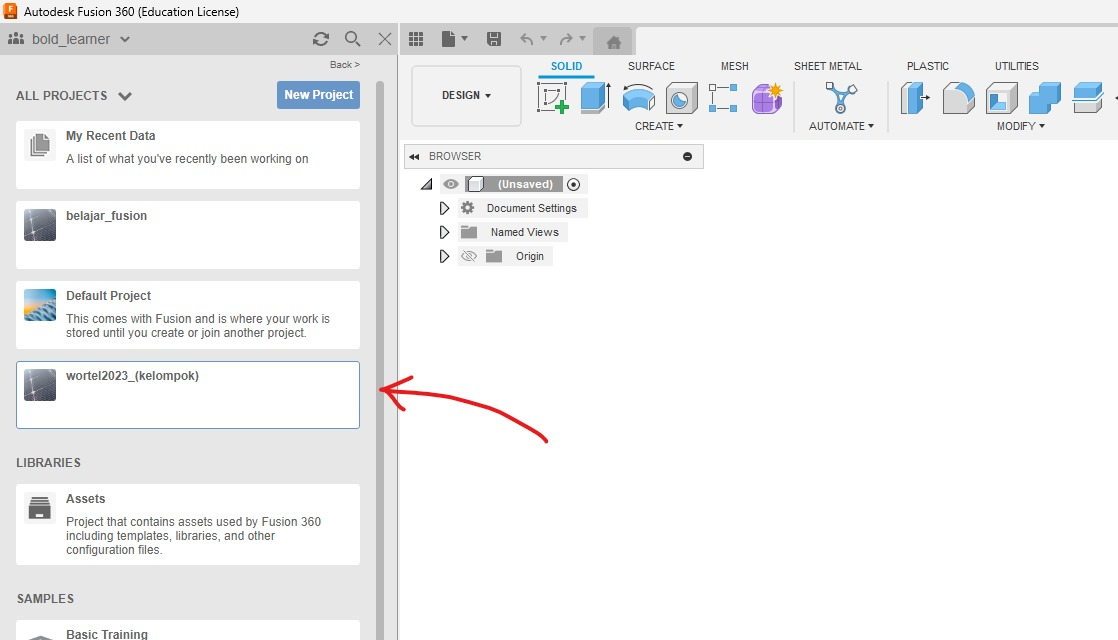
\includegraphics[width=0.6\linewidth]{P1/img/gambar2.jpeg}
            \caption{buka project} 
            \label{fig:buka project}
        \end{figure}
    \item Sebelum memulai mengerjakan pada project, kita harus mengimport library yang berisi semua komponen yang diperlukan. Klik \textbf{File > Open}
        \begin{figure}[H]
            \centering
            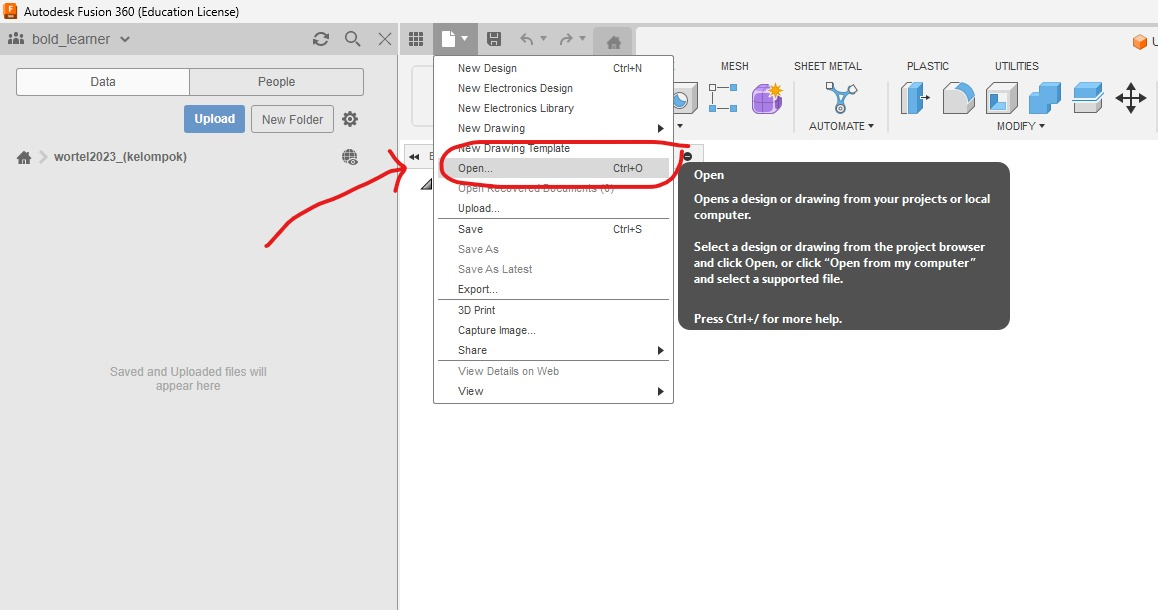
\includegraphics[width=0.6\linewidth]{P1/img/gambar3.jpeg}
            \caption{Membuka prompt File Select} 
            \label{fig:Membuka prompt File Select}
        \end{figure}
    Selanjutnya pilih \textbf{Open from my computer}
    \begin{figure}[H]
        \centering
        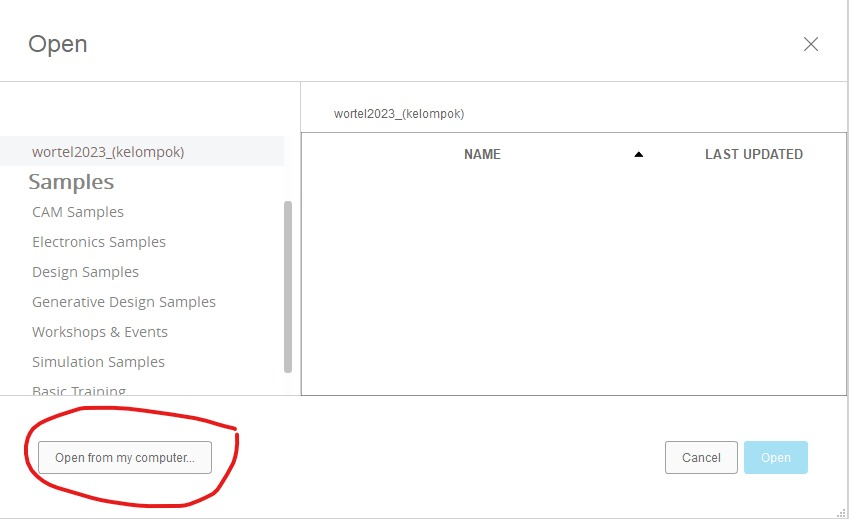
\includegraphics[width=0.6\linewidth]{P1/img/gambar4.jpeg}
        \caption{Mengakses file di Komputer} 
        \label{fig:Mengakses file di Komputer}
    \end{figure}
    Cari dimana file library untuk modul ini tersimpan pada folder file anda, file tersebut memiliki extensi file .lbr
    \begin{figure}[H]
        \centering
        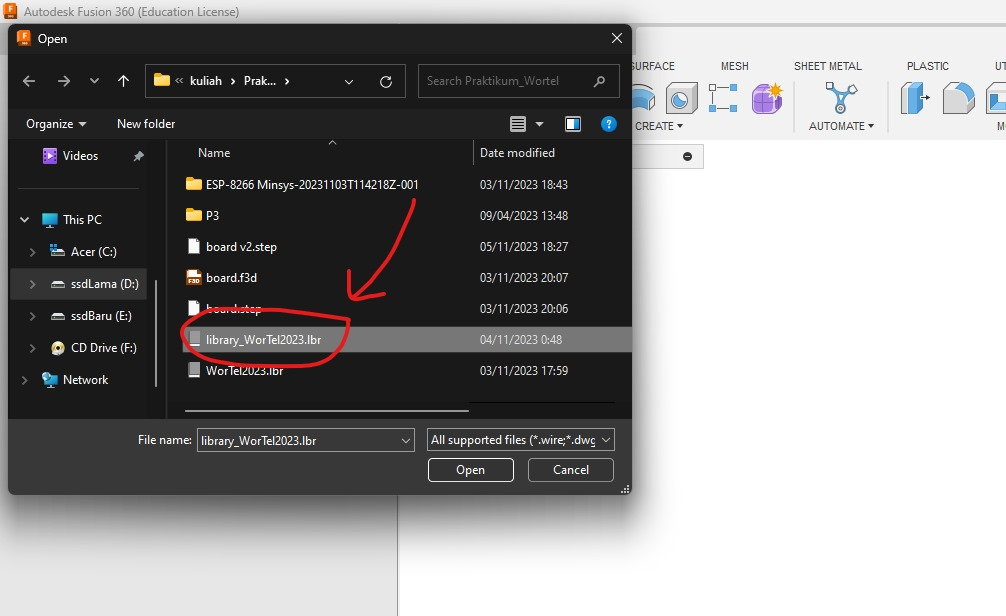
\includegraphics[width=0.6\linewidth]{P1/img/gambar5.jpeg}
        \caption{Memilih Library} 
        \label{fig:Memilih Library}
    \end{figure}
    Setelah library terimport, klik \textbf{ctrl + S} untuk melakukan saving library pada project yang anda miliki dan klik save.
    \begin{figure}[H]
        \centering
        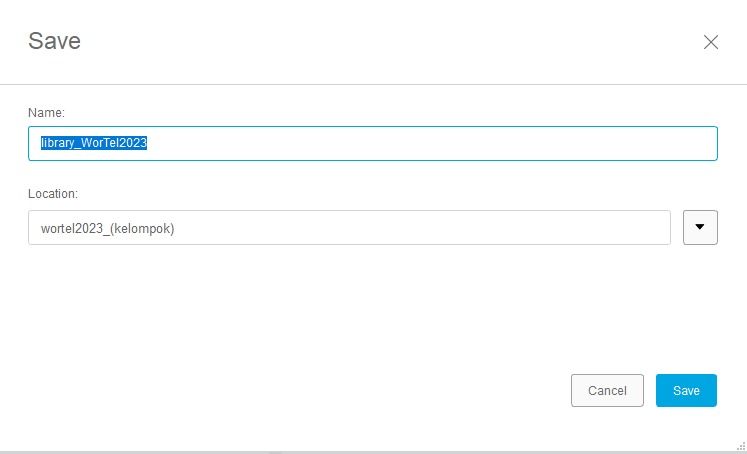
\includegraphics[width=0.6\linewidth]{P1/img/gambar6.jpeg}
        \caption{Simpan Library} 
        \label{fig:Simpan Library}
    \end{figure}
    Maka tampilan Fusion anda akan menjadi seperti \textbf{Gambar 1.7}, dimana telah terdapat list komponen yang anda perlukan.
        \begin{figure}[H]
            \centering
            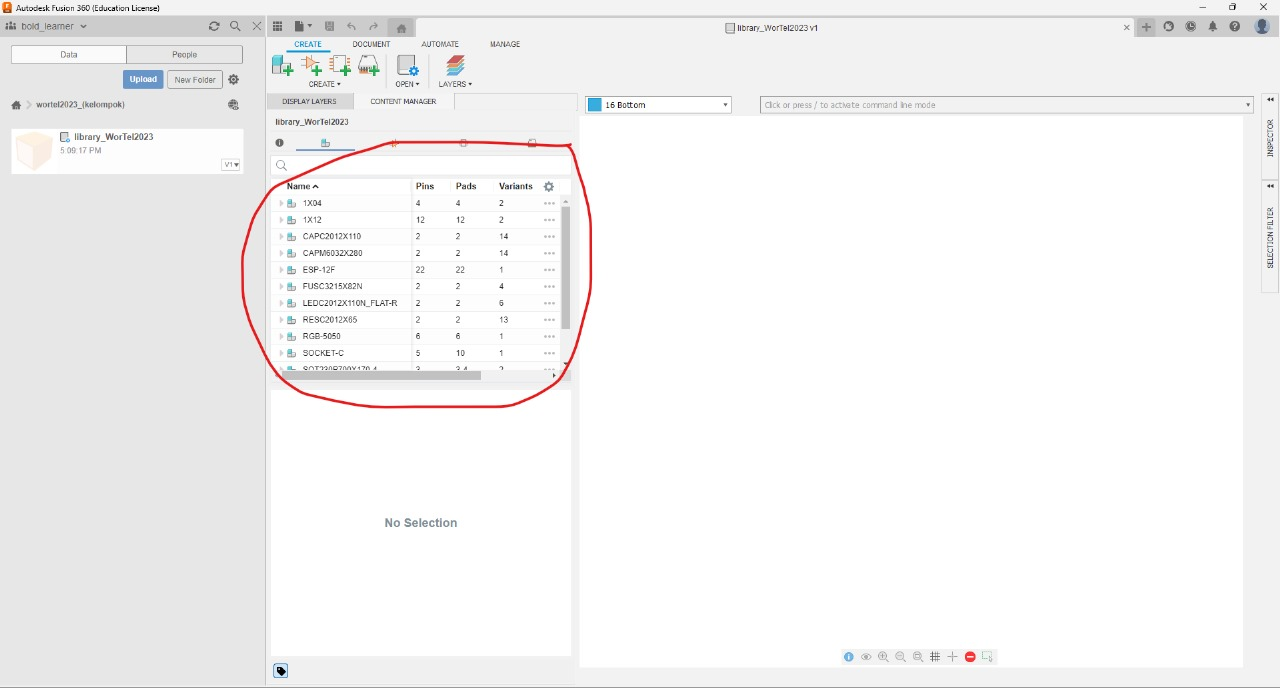
\includegraphics[width=0.6\linewidth]{P1/img/gambar7.jpeg}
            \caption{Tampilan Fusion} 
            \label{fig:TampilanFusion1}
        \end{figure}
    \item Berikutnya untuk memulai mendesign rangkaian, klik \textbf{File > New Electonic Design}
        \begin{figure}[H]
            \centering
            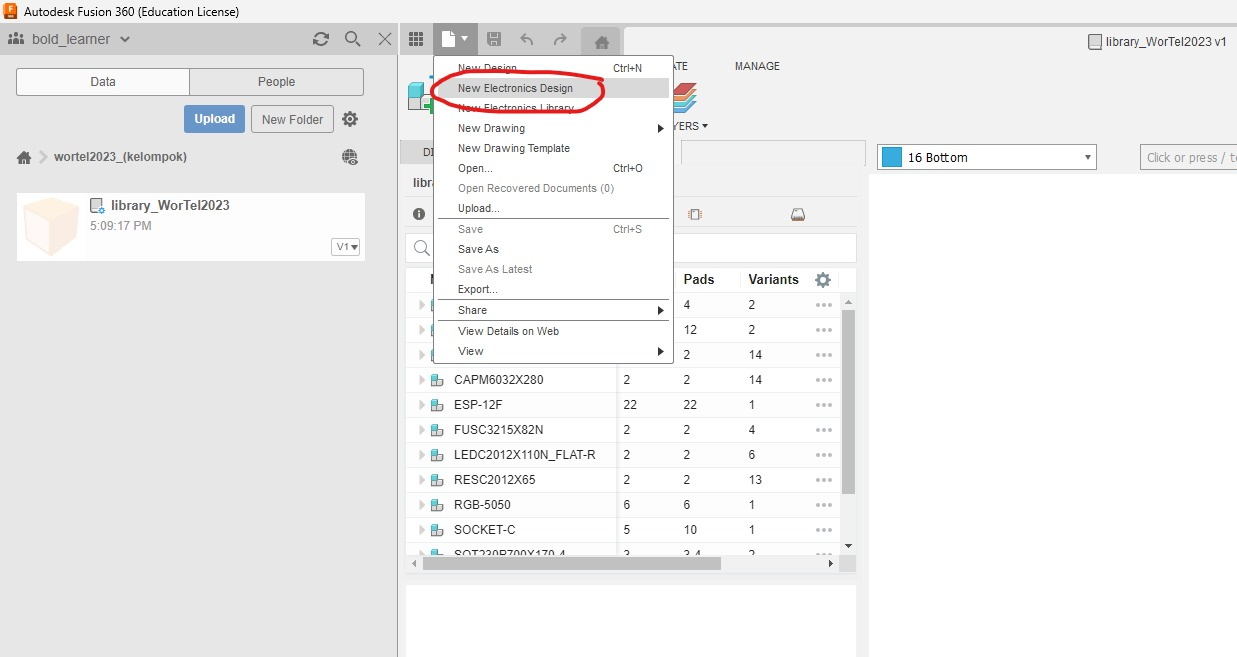
\includegraphics[width=0.6\linewidth]{P1/img/gambar8.jpeg}
            \caption{Memulai desain rangkaian} 
            \label{fig:Memulai desain rangkaian}
        \end{figure}
    Lakukan penyimpanan dengan menekan \textbf{ctrl + S} lalu beri nama sesuai keinginan kalian.
        \begin{figure}[H]
            \centering
            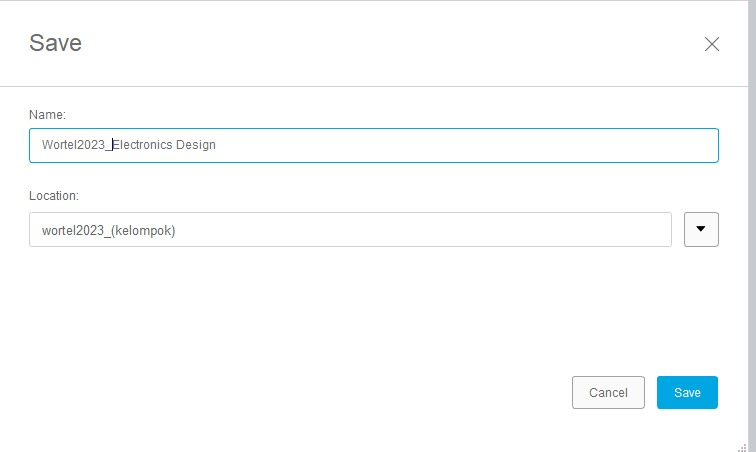
\includegraphics[width=0.6\linewidth]{P1/img/gambar9.jpeg}
            \caption{Menyimpan workspace} 
            \label{fig:Menyimpan workspace}
        \end{figure}
    Tampilan Fusion anda akan menjadi seperti \textbf{gambar 1.10}
        \begin{figure}[H]
            \centering
            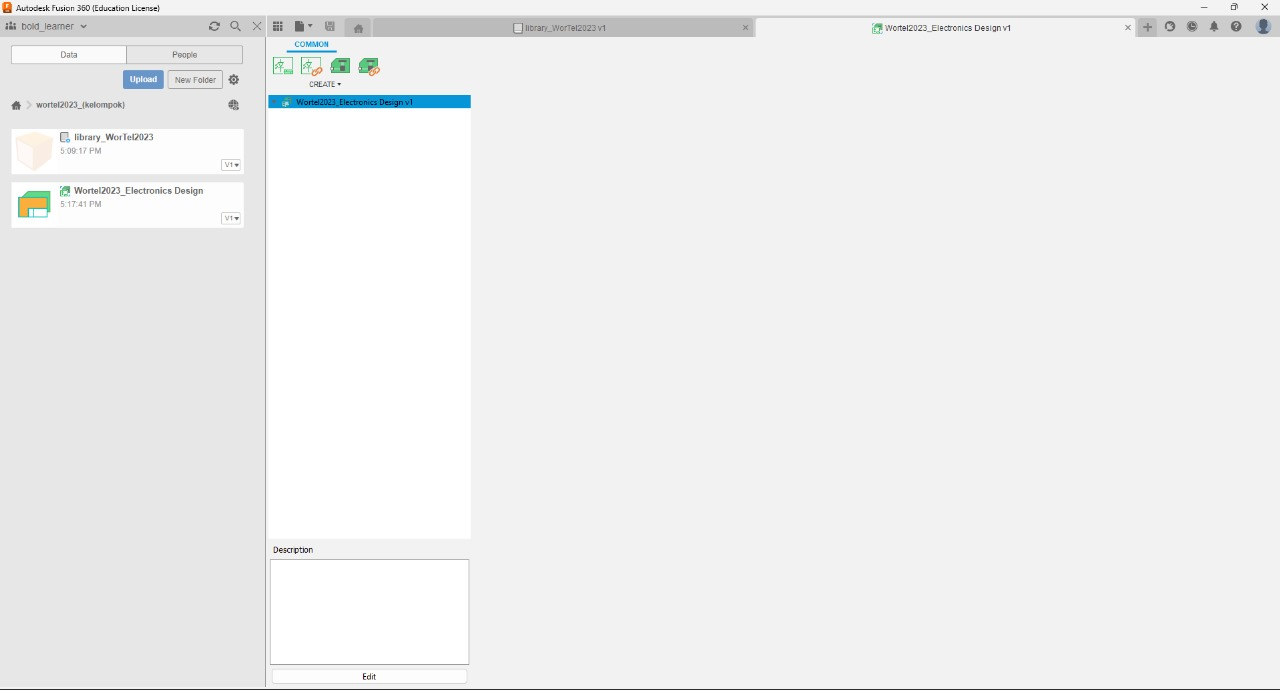
\includegraphics[width=0.6\linewidth]{P1/img/gambar10.jpeg}
            \caption{Tampilan Fusion} 
            \label{fig:Tampilan Fusion}
        \end{figure}
    \item Untuk membuat lembar schematic dan mulai mendesain, klik tombol \textbf{New Schematic} 
        \begin{figure}[H]
            \centering
            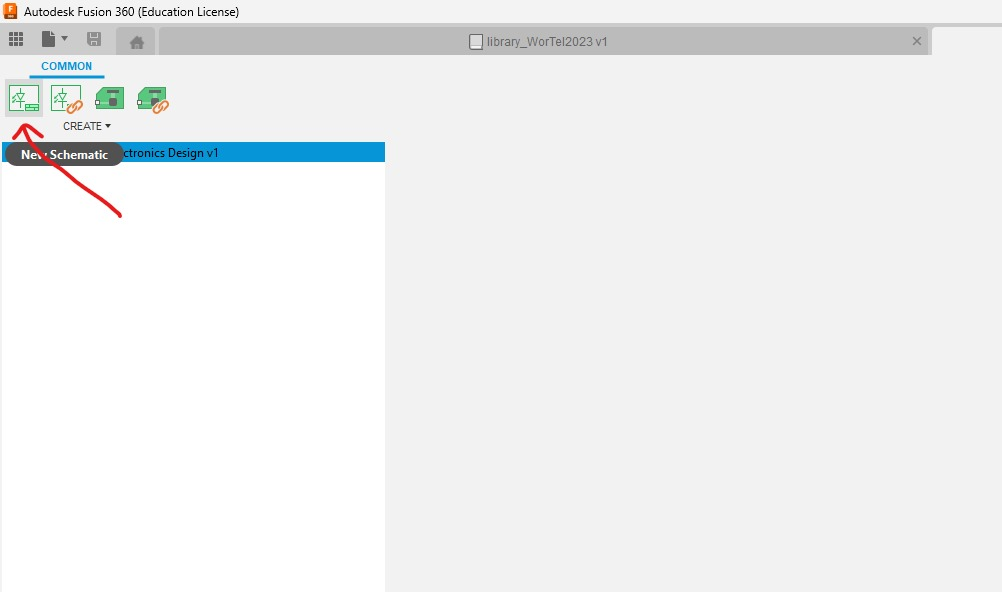
\includegraphics[width=0.6\linewidth]{P1/img/gambar11.jpeg}
            \caption{New Schmatic} 
            \label{fig:New Schematic}
        \end{figure}
    berikutnya tekan \textbf{ctrl + S} lalu beri nama dan simpan schematic.
    \item Untuk meletakan komponen, dapat menggunakan tool \textbf{Place Component} yang terletak pada bagian dari Fusion.
        \begin{figure}[H]
            \centering
            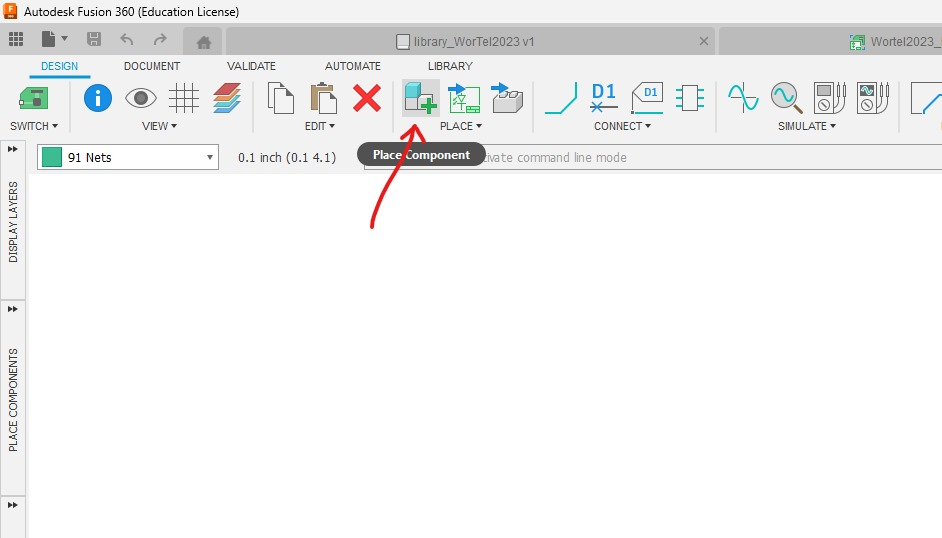
\includegraphics[width=0.6\linewidth]{P1/img/gambar13.jpeg}
            \caption{Place Component} 
            \label{fig:Place Component}
        \end{figure}
    \item Tekan icon \textbf{Open Library Manager} sesuai dengan \textbf{gambar 1.14}
        \begin{figure}[H]
            \centering
            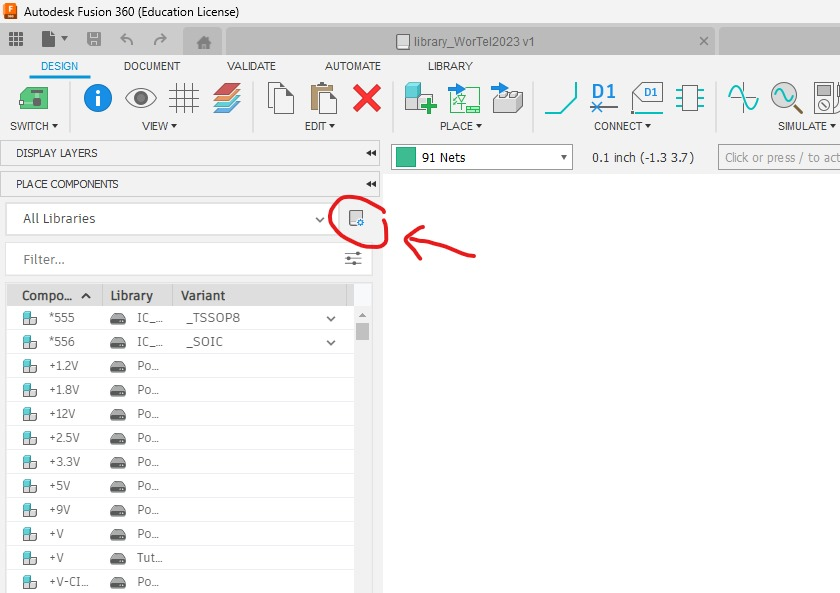
\includegraphics[width=0.6\linewidth]{P1/img/gambar14.jpeg}
            \caption{Membuka Library Manager} 
            \label{fig:Membuka LIbrary Manager}
        \end{figure}
    Berikutnya aktifkan library yang sebelumnya telah anda tambahkan dan pastikan statusnya \textbf{In Use}
        \begin{figure}[H]
            \centering
            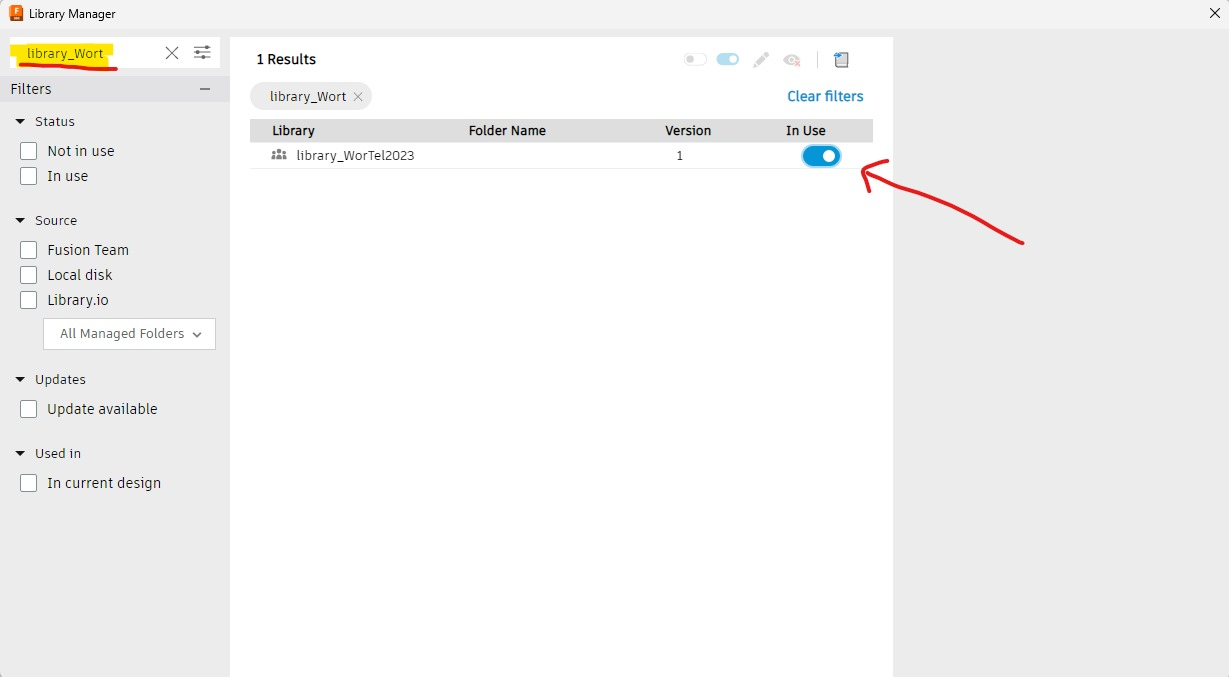
\includegraphics[width=0.6\linewidth]{P1/img/gambar15.jpeg}
            
            
            \label{fig:Status Library}
        \end{figure}
    \item Berikut adalah komponen-komponen yang anda butuhkan :
    \vspace{5pt}
    \begin{table}[ht]
        
   
    \begin{center}
    
        \caption{Komponen}
        \label{tab:komponen}

        \begin{tabular}{|c|p{2cm}|m{2cm}|m{2cm}|m{2cm}|}
            \hline
            Gambar & Nama & Library & Jumlah & Catatan \\
            \hline
            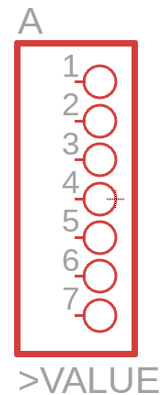
\includegraphics[width=0.05\linewidth]{P1/img/Header_1x7_2.png} &  {\fontsize{8}{6}\selectfont HEADER 1x7} &  {\fontsize{8}{6}\selectfont WorTel Library} & 1 & - \\
            \hline
            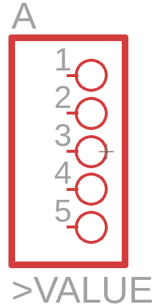
\includegraphics[width=0.05\linewidth]{P1/img/Header_1x5_2.png} & {\fontsize{8}{6}\selectfont HEADER 1X5} & {\fontsize{8}{6}\selectfont WorTel Library} & 1 &  - \\
            \hline
            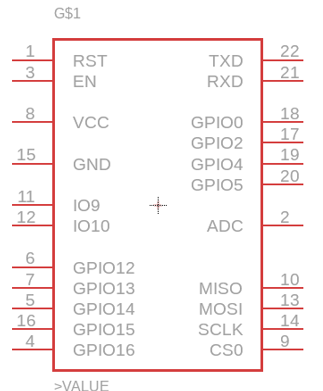
\includegraphics[width=0.05\linewidth]{P1/img/ESP-12F_2.png} & {\fontsize{8}{6}\selectfont ESP-12F} & {\fontsize{8}{6}\selectfont WorTel Library} & 1 &  - \\
            \hline
            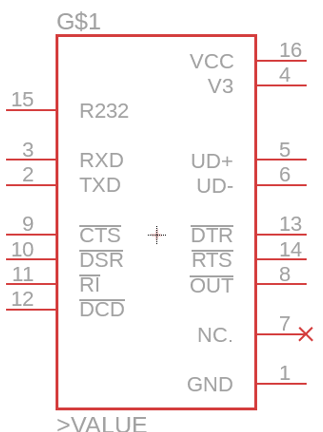
\includegraphics[width=0.05\linewidth]{P1/img/CH340_2.png} & {\fontsize{8}{6}\selectfont CH340} &  {\fontsize{8}{6}\selectfont WorTel Library} & 1 & - \\
            \hline
            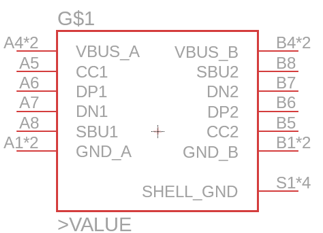
\includegraphics[width=0.05\linewidth]{P1/img/USB-C_2.png} & {\fontsize{8}{6}\selectfont USB-C} &  {\fontsize{8}{6}\selectfont WorTel Library} & 1 & - \\
            \hline
            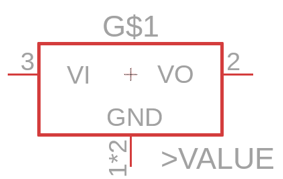
\includegraphics[width=0.05\linewidth]{P1/img/Regulator_3V3_2.png} & {\fontsize{8}{6}\selectfont Regulator 3V3} &  {\fontsize{8}{6}\selectfont WorTel Library} & 1 & - \\
            \hline
            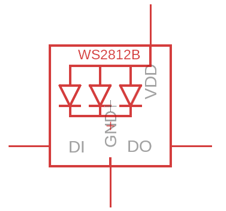
\includegraphics[width=0.1\linewidth]{P1/img/WS2812B_2.png} & {\fontsize{8}{6}\selectfont WS2812B} &  {\fontsize{8}{6}\selectfont WorTel Library} & 1 & - \\
            \hline
            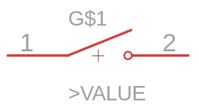
\includegraphics[width=0.1\linewidth]{P1/img/Button_2.png} & {\fontsize{8}{6}\selectfont Button} &  {\fontsize{8}{6}\selectfont WorTel Library} & 2 & - \\
            \hline
            
\includegraphics[width=0.1\linewidth]{P1/img/Capacitor_2.png} & {\fontsize{8}{6}\selectfont Capacitor} &  {\fontsize{8}{6}\selectfont WorTel Library} & 5 & {\fontsize{8}{6}\selectfont 100uF(3), 100nf(1), 1uF(1)} \\
            \hline
            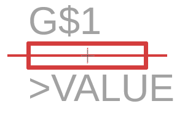
\includegraphics[width=0.1\linewidth]{P1/img/Fuse_2.png} & {\fontsize{8}{6}\selectfont Fuse} &  {\fontsize{8}{6}\selectfont WorTel Library} & 1 & - \\
            \hline
            
\includegraphics[width=0.1\linewidth]{P1/img/LED_2.png} & {\fontsize{8}{6}\selectfont LED} &  {\fontsize{8}{6}\selectfont WorTel Library} & 1 & - \\
            \hline
            
\includegraphics[width=0.1\linewidth]{P1/img/NMOSFET_2.png} & {\fontsize{8}{6}\selectfont NMOSFET} &  {\fontsize{8}{6}\selectfont WorTel Library} & 2 & - \\
            \hline
            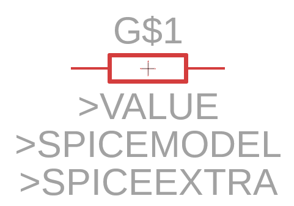
\includegraphics[width=0.1\linewidth]{P1/img/RESISTOR_2.png} & {\fontsize{8}{6}\selectfont Resistor} &  {\fontsize{8}{6}\selectfont WorTel Library} & 7 & {\fontsize{8}{6}\selectfont 10k(4), 5.1k(2), 1k(1)} \\
            \hline
            \end{tabular}
        \vspace{-\topsep} % Mengurangi spasi sebelum tabel
    \end{center}
\end{table}
    \vspace{5pt}
    \\
    \\
    \item Sambungkan seluruh komponen dengan koneksi pin.
    \item Hasil dari rangkaian dari Minimum System ESP8266 adalah sebagai berikut :
        \begin{figure}[H]
            \centering
            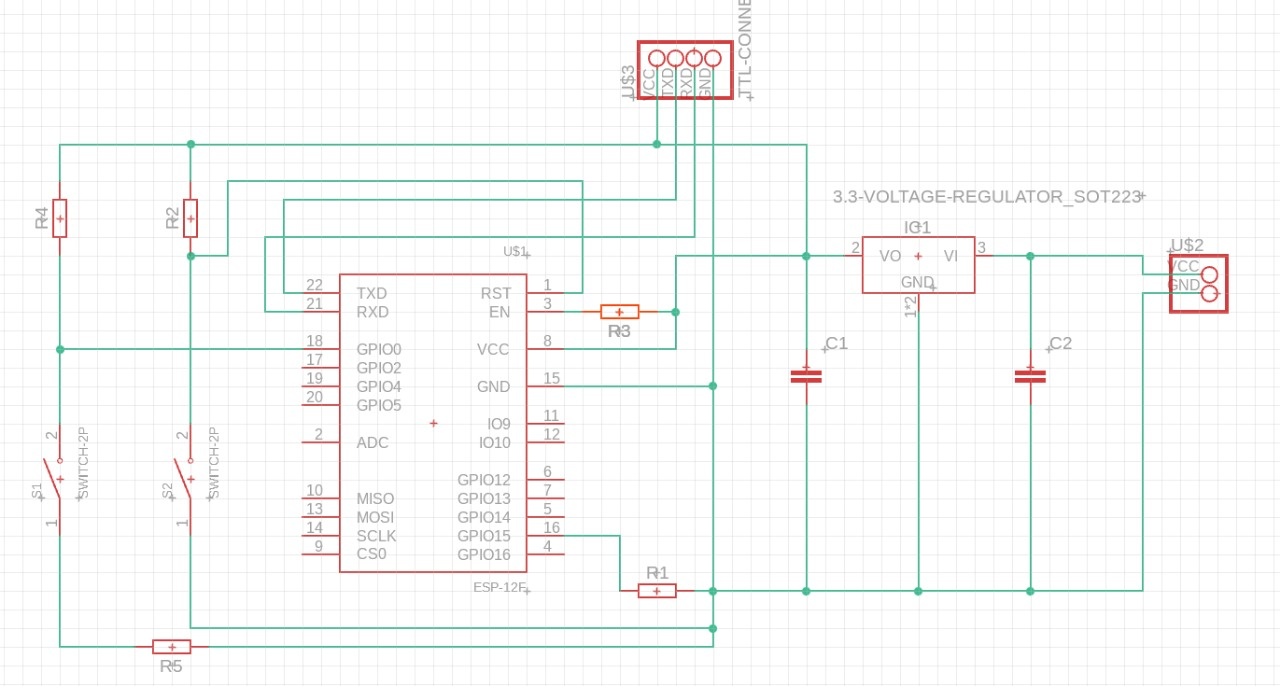
\includegraphics[width=0.6\linewidth]{P1/img/gambar23.jpg}
            \caption{Hasil Rangkaian} 
            \label{fig:Hasil Rangkaian}
        \end{figure}
\end{enumerate}

\section{Alat dan Komponen}
\subsection{Alat}
\begin{enumerate}
    \item Laptop yang telah terinstall Autodesk Fusion 360
    \item Mouse
\end{enumerate}

\section{Eksperimen 1: PCB design Minimum System ESP8266}
Setelah proses penyusunan schematic selesai, waktunya mendesain bagaimana Printed Circuit Board
dari schematic tersebut akan tersusun.
\begin{enumerate}
    \item Untuk melanjutkan mendesain board dari schematic gunakan tools \textbf{“Switch to PCB
    documentation”}
    \begin{figure}[H]
        \centering
        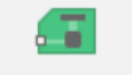
\includegraphics[width=0.4\linewidth]{P1/img/switchtopcb.png}
        \caption{Switch to PCB} 
        \label{fig:Switch to PCB}
    \end{figure}
    Pada bagian awal saat mengubah ke board, akan disuguhkan tampilan sebagai berikut. Pada
    bagian kiri terdapat Footprint dari komponen dengan garis warna kuning yang
    menghubungkan antar footprint komponen sesuai dengan wiring pada schematic. Pada
    bagian kanan terdapat “Board” yang berbentuk persegi hitam yaitu tempat untuk meletakan
    footprint komponen.
    \begin{figure}[H]
        \centering
        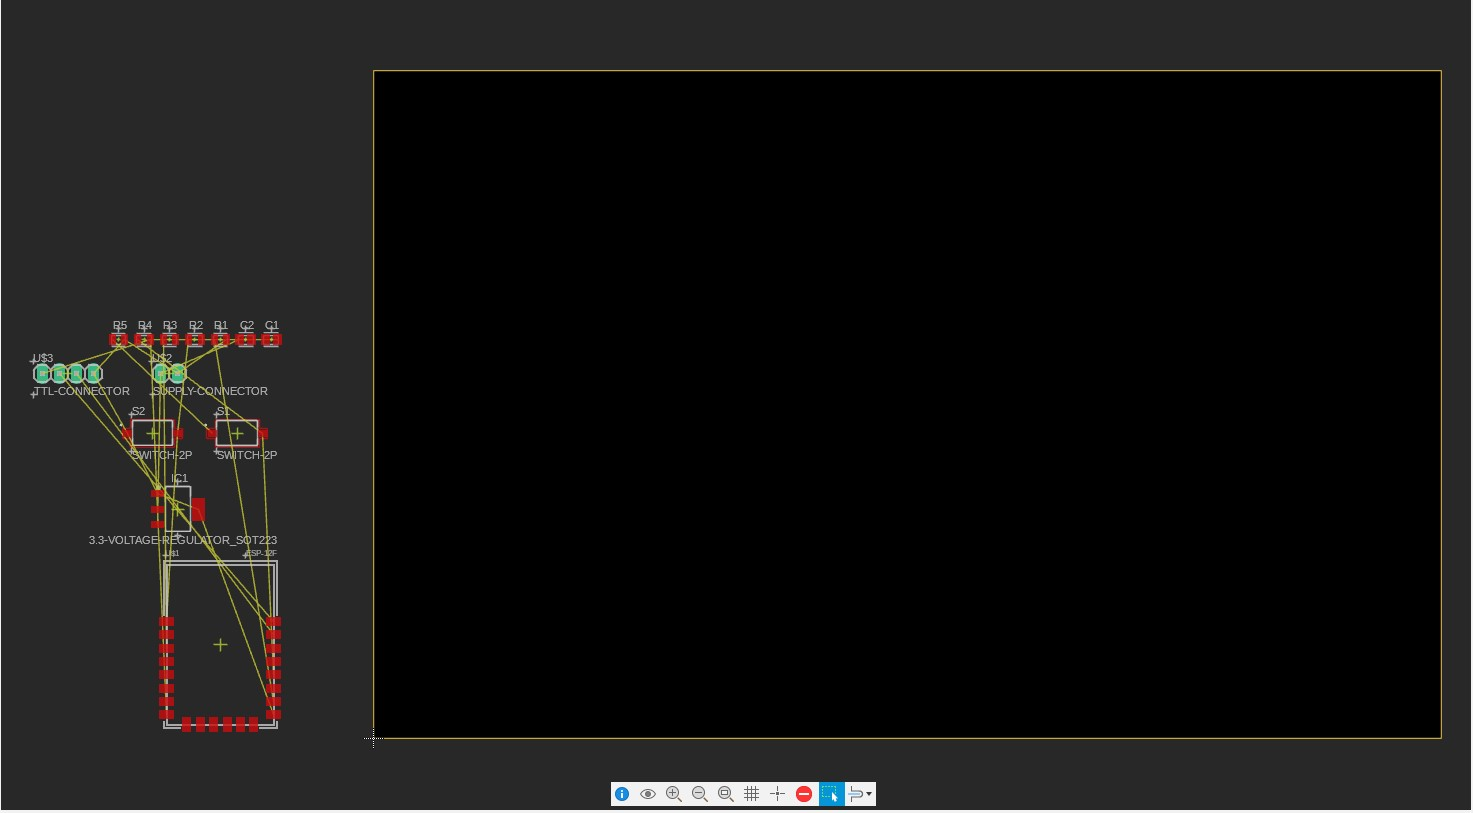
\includegraphics[width=0.6\linewidth]{P1/img/awal_switch_ke_pcb_design.jpg}
        \caption{PCB awal} 
        \label{fig:PCBawal}
    \end{figure}
    \vspace{-\topsep}
    \item Masukan seluruh footprint komponen ke dalam Board dengan memilih seluruh footprint menggunakan tools \textbf{Group} dan digerakan dengan menggukan tools \textbf{Move}.
    \begin{figure}[H]
        \centering
        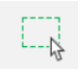
\includegraphics[width=0.15\linewidth]{P1/img/group.png}
        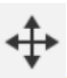
\includegraphics[width=0.12\linewidth]{P1/img/move.png}
        \caption{Group dan Move}
    \end{figure}
    \begin{figure}[H]
        \centering
        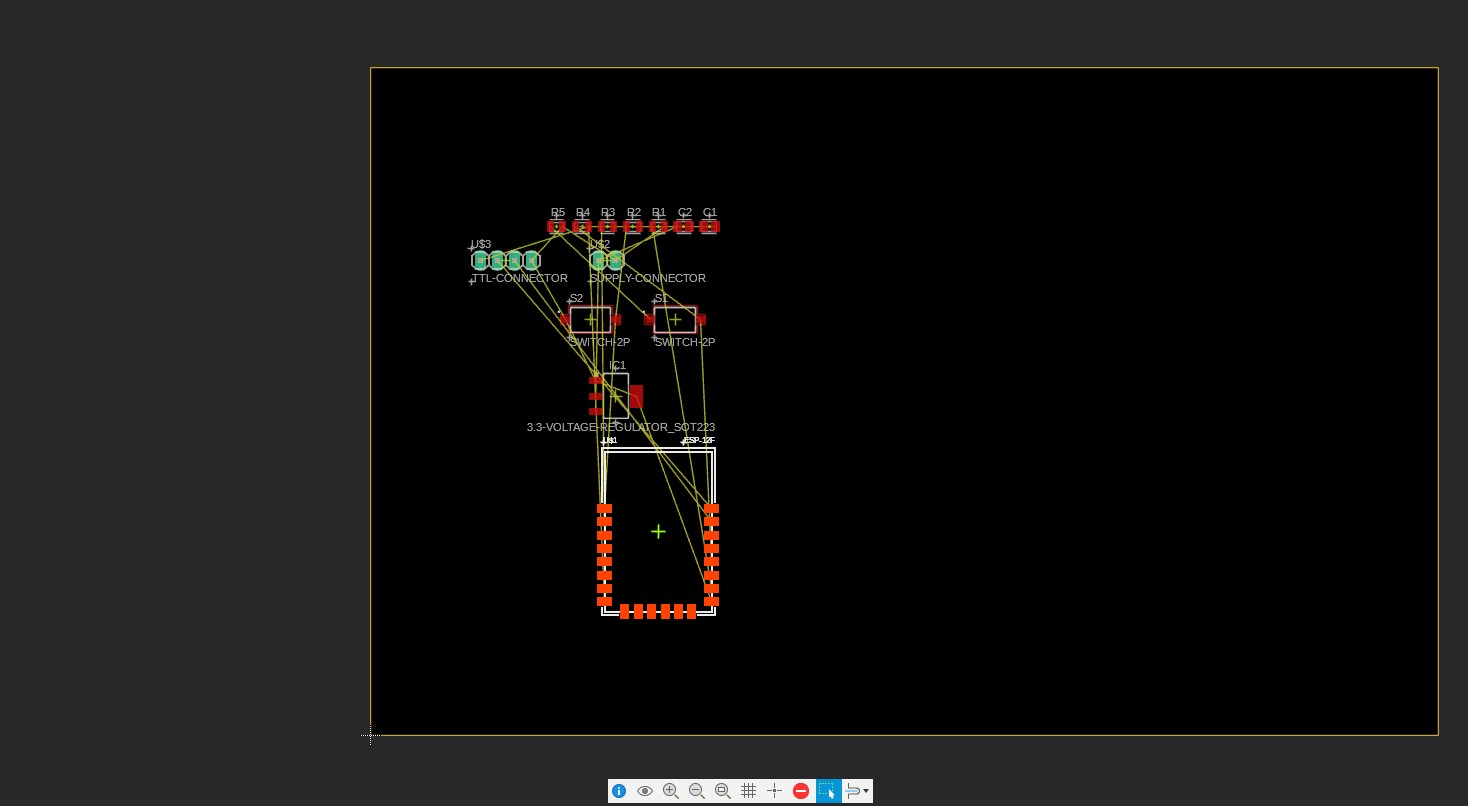
\includegraphics[width=0.6\linewidth]{P1/img/masukkan_semua_komponen_ke_lingkup_pcb.jpg}
        \caption{Hasil setelah dipindah} 
        \label{fig:Hasil setelah dipindah}
    \end{figure}
    \item Susun footprint serapi mungkin dengan mengerakan footprint menggunakan tools
    \textbf{Move}
        \begin{figure}[H]
            \centering
            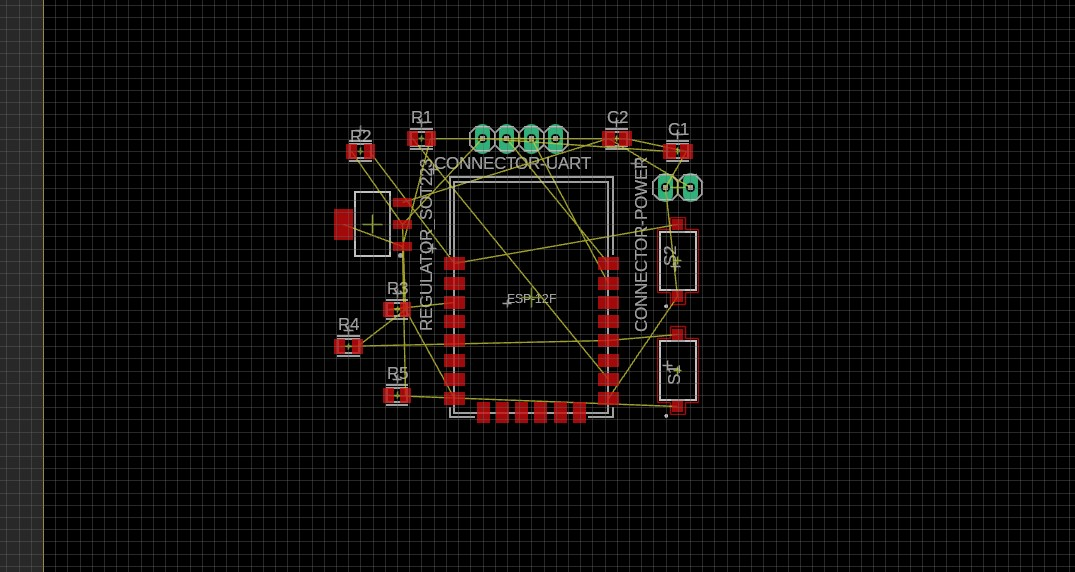
\includegraphics[width=0.6\linewidth]{P1/img/rapihkan_tatanan_komponen.jpg}
            \caption{PCB awal} 
            \label{fig:PCB awal}
        \end{figure}
    \item Raphikan tatanan komponen serta atur ukuran “Board” dengan menggerakan/geser garis tepi dari “Board” hingga ukuran
    sesuai dengan tatanan footprint.
        \begin{figure}[H]
            \centering
            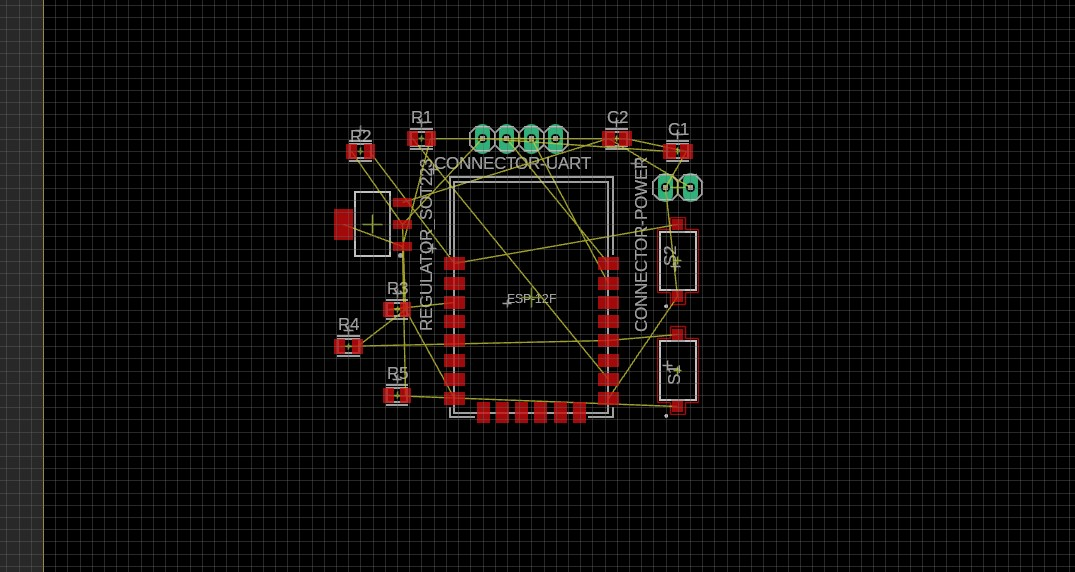
\includegraphics[width=0.5\linewidth]{P1/img/rapihkan_tatanan_komponen.jpg}
            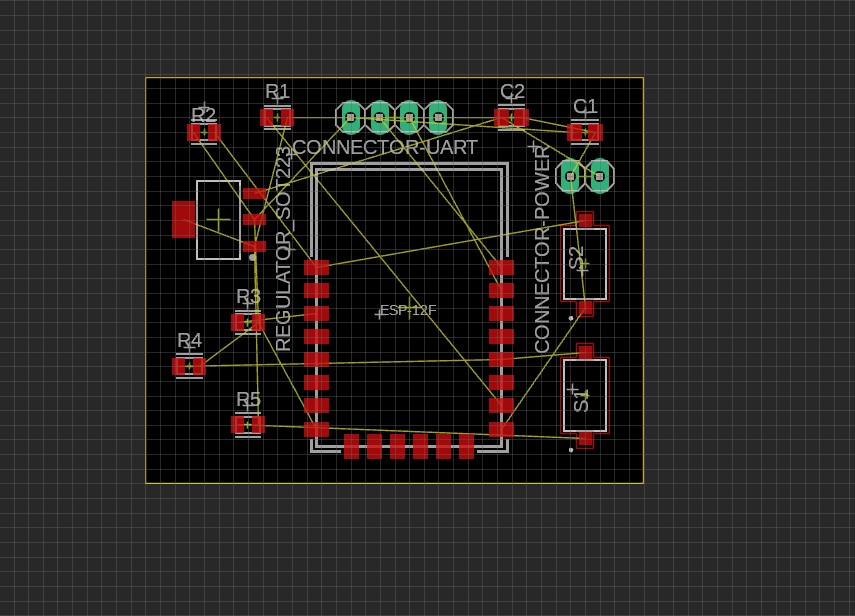
\includegraphics[width=0.45\linewidth]{P1/img/hasil_rapi.jpg}
            \caption{Setelah board dikecilkan} 
            \label{fig:Setelah komponen dirapihkan dan dikecilkan}
        \end{figure}
    \item Selanjutnya adalah melakukan routing jalur koneksi. Dalam melakukan Routing, Tools
    utama yang digunakan adalah \textbf{Route Manual} dan \textbf{Unroute} untuk
    menghapus route. Jalur Routing mengikuti garis warna kuning.
        \begin{figure}[H]
            \centering
            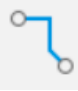
\includegraphics[width=0.12\linewidth]{P1/img/manualroute.png}
            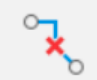
\includegraphics[width=0.17\linewidth]{P1/img/unroute.png}
            \caption{Manual route dan unroute}
        \end{figure}
        \begin{figure}[H]
            \centering
            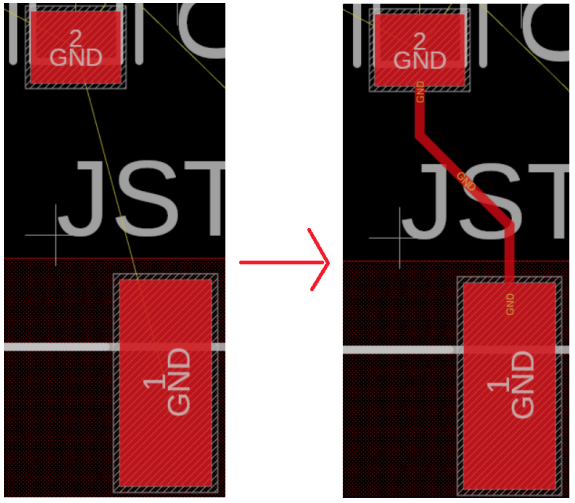
\includegraphics[width=0.89\linewidth]{P1/img/routing1.png}
            \caption{Contoh cara routing}
        \end{figure}
    \item Saat menggunakan Routing normalnya layer yang digunakan adalah \textbf{1 Top} akan tetapi
    Routing yang dibuat di layer yang sama tidak bisa saling ditabrak/ tumpuk.
        \begin{figure}[H]
            \centering
            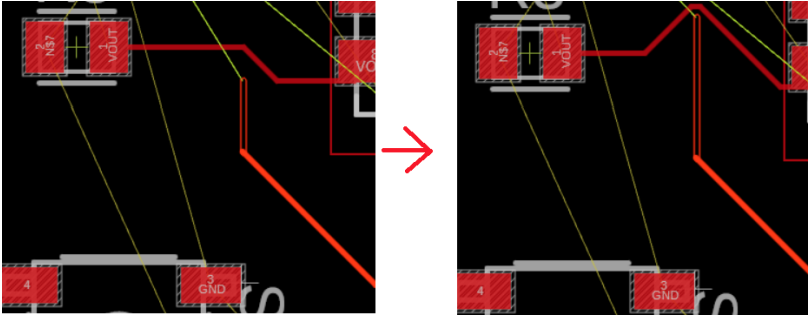
\includegraphics[width=0.89\linewidth]{P1/img/routing2.png}
            \caption{Contoh routing routing yang bertabrakan}
        \end{figure}
    Maka untuk mengatasi hal itu dapat digunakan layer yang lain. Untuk berpindah layer
    menjadi \textbf{16 Bottom} saat menggunakan Route Manual dapat di klik mouse 3 (scroll wheel)
    untuk meletakan \textbf{Vias} yaitu lingkaran penghubung layer top dan bottom. Berpindah layer
    berfungsi agar jalur routing tidak bertabrakan.
        \begin{figure}[H]
            \centering
            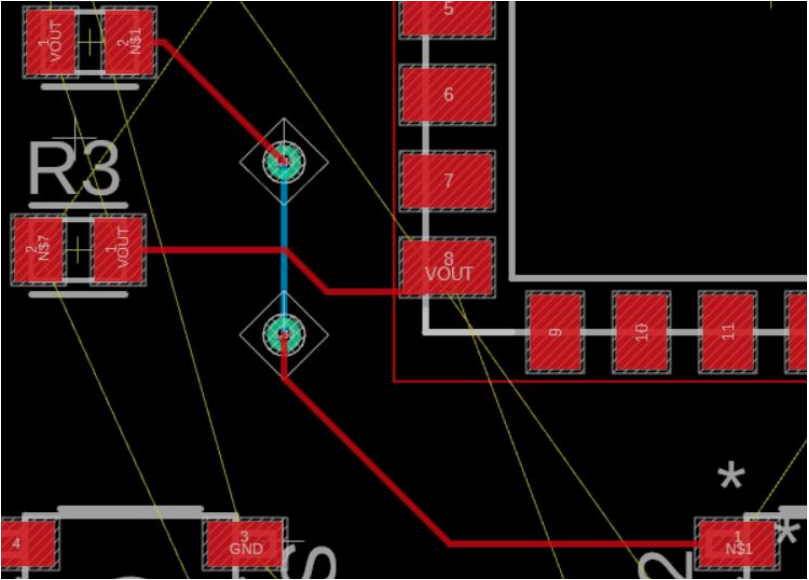
\includegraphics[width=0.89\linewidth]{P1/img/routing3.png}
            \caption{Vias yang menghubungkan Routing top(merah) dengan Bottom(biru)}
        \end{figure}
    \item Routing Seluruh garis koneksi warna kuning hingga seluruhnya tersambung. \textbf{
    Pastikan jalur Routing tidak saling berdekatan dengan jalur lain.}
        \begin{figure}[H]
            \centering
            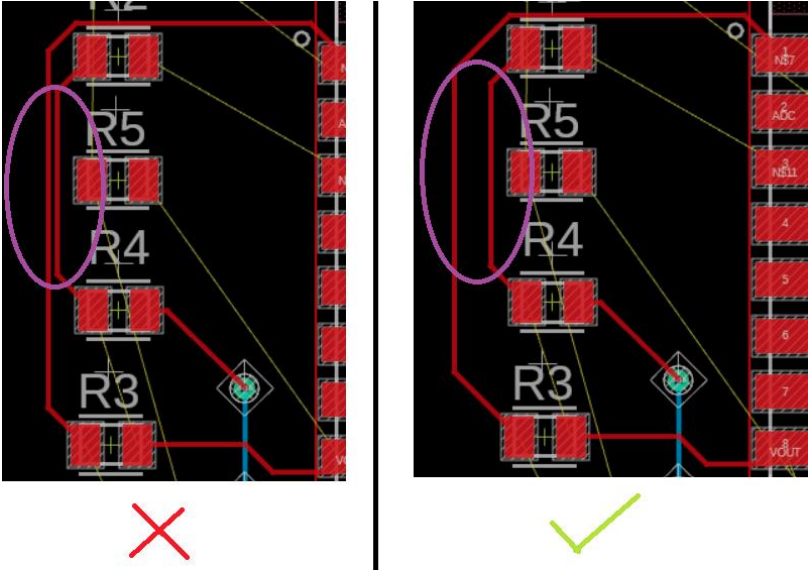
\includegraphics[width=0.89\linewidth]{P1/img/routing4.png}
            \caption{Contoh rangkaian yang tidak bagus dan bagus}
        \end{figure}

    \item Setelah selesai klik save (ctrl+s).
    \textbf{Contoh rangkaian PCB yang sudah jadi :}
        \begin{figure}[H]
            \centering
            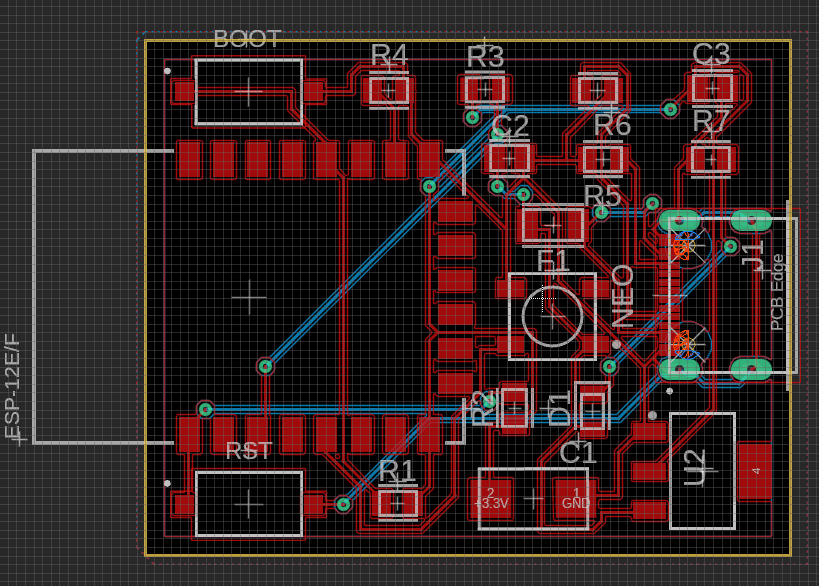
\includegraphics[width=0.47\linewidth]{P1/img/gambar_jadi.jpg}
            \caption{Hasil sesudah di routing}
        \end{figure}
\end{enumerate}